\clearpage 
\section*{\underline{Extended Data}}

%\renewcommand\thefigure{\thesection.\arabic{figure}}    
\setcounter{figure}{0}    

\begin{figure}[h!]
	\centering
	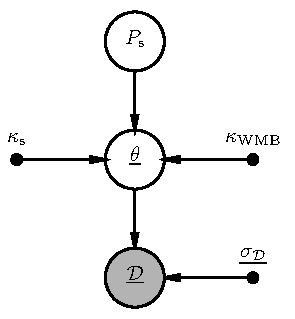
\includegraphics[width=0.6 \textwidth]{pgm_models.pdf}
	\caption{A probabilistic graphical model (PGM) represented algebraically in Equation \ref{eq:modelll}. The shaded circle indicates observed data, and solid black points represent other fixed information, such as the KDEs and observational uncertainties. The remaining circles represent parameters. The underline indicates that the symbol represents a set of parameters or data. Here, $\kappa_{\rm{s}}$ and $\kappa_{\rm WMB}$ represent the KDEs of standard and WMB model populations respectively. $P_{\rm{s}}$ is the mixture model weighting factor. The latent parameters $\underline{\theta}$, our observations $\underline{\mathcal{D}}$ and their uncertainties $\underline{\sigma_{\mathcal{D}}}$ include temperature (\teff), mass ($M$), log-age ($\ln(t)$), metallicity (\feh) and log-rotation ($\ln(P)$). This model is \textit{hierarchical}, as all the latent parameters are drawn from the common probability distribution set by $P_{\rm{s}}$ and described in Equation \ref{eq:mixturell}.}
	\label{fig:pgm}
\end{figure}

\begin{figure}
	\centering
	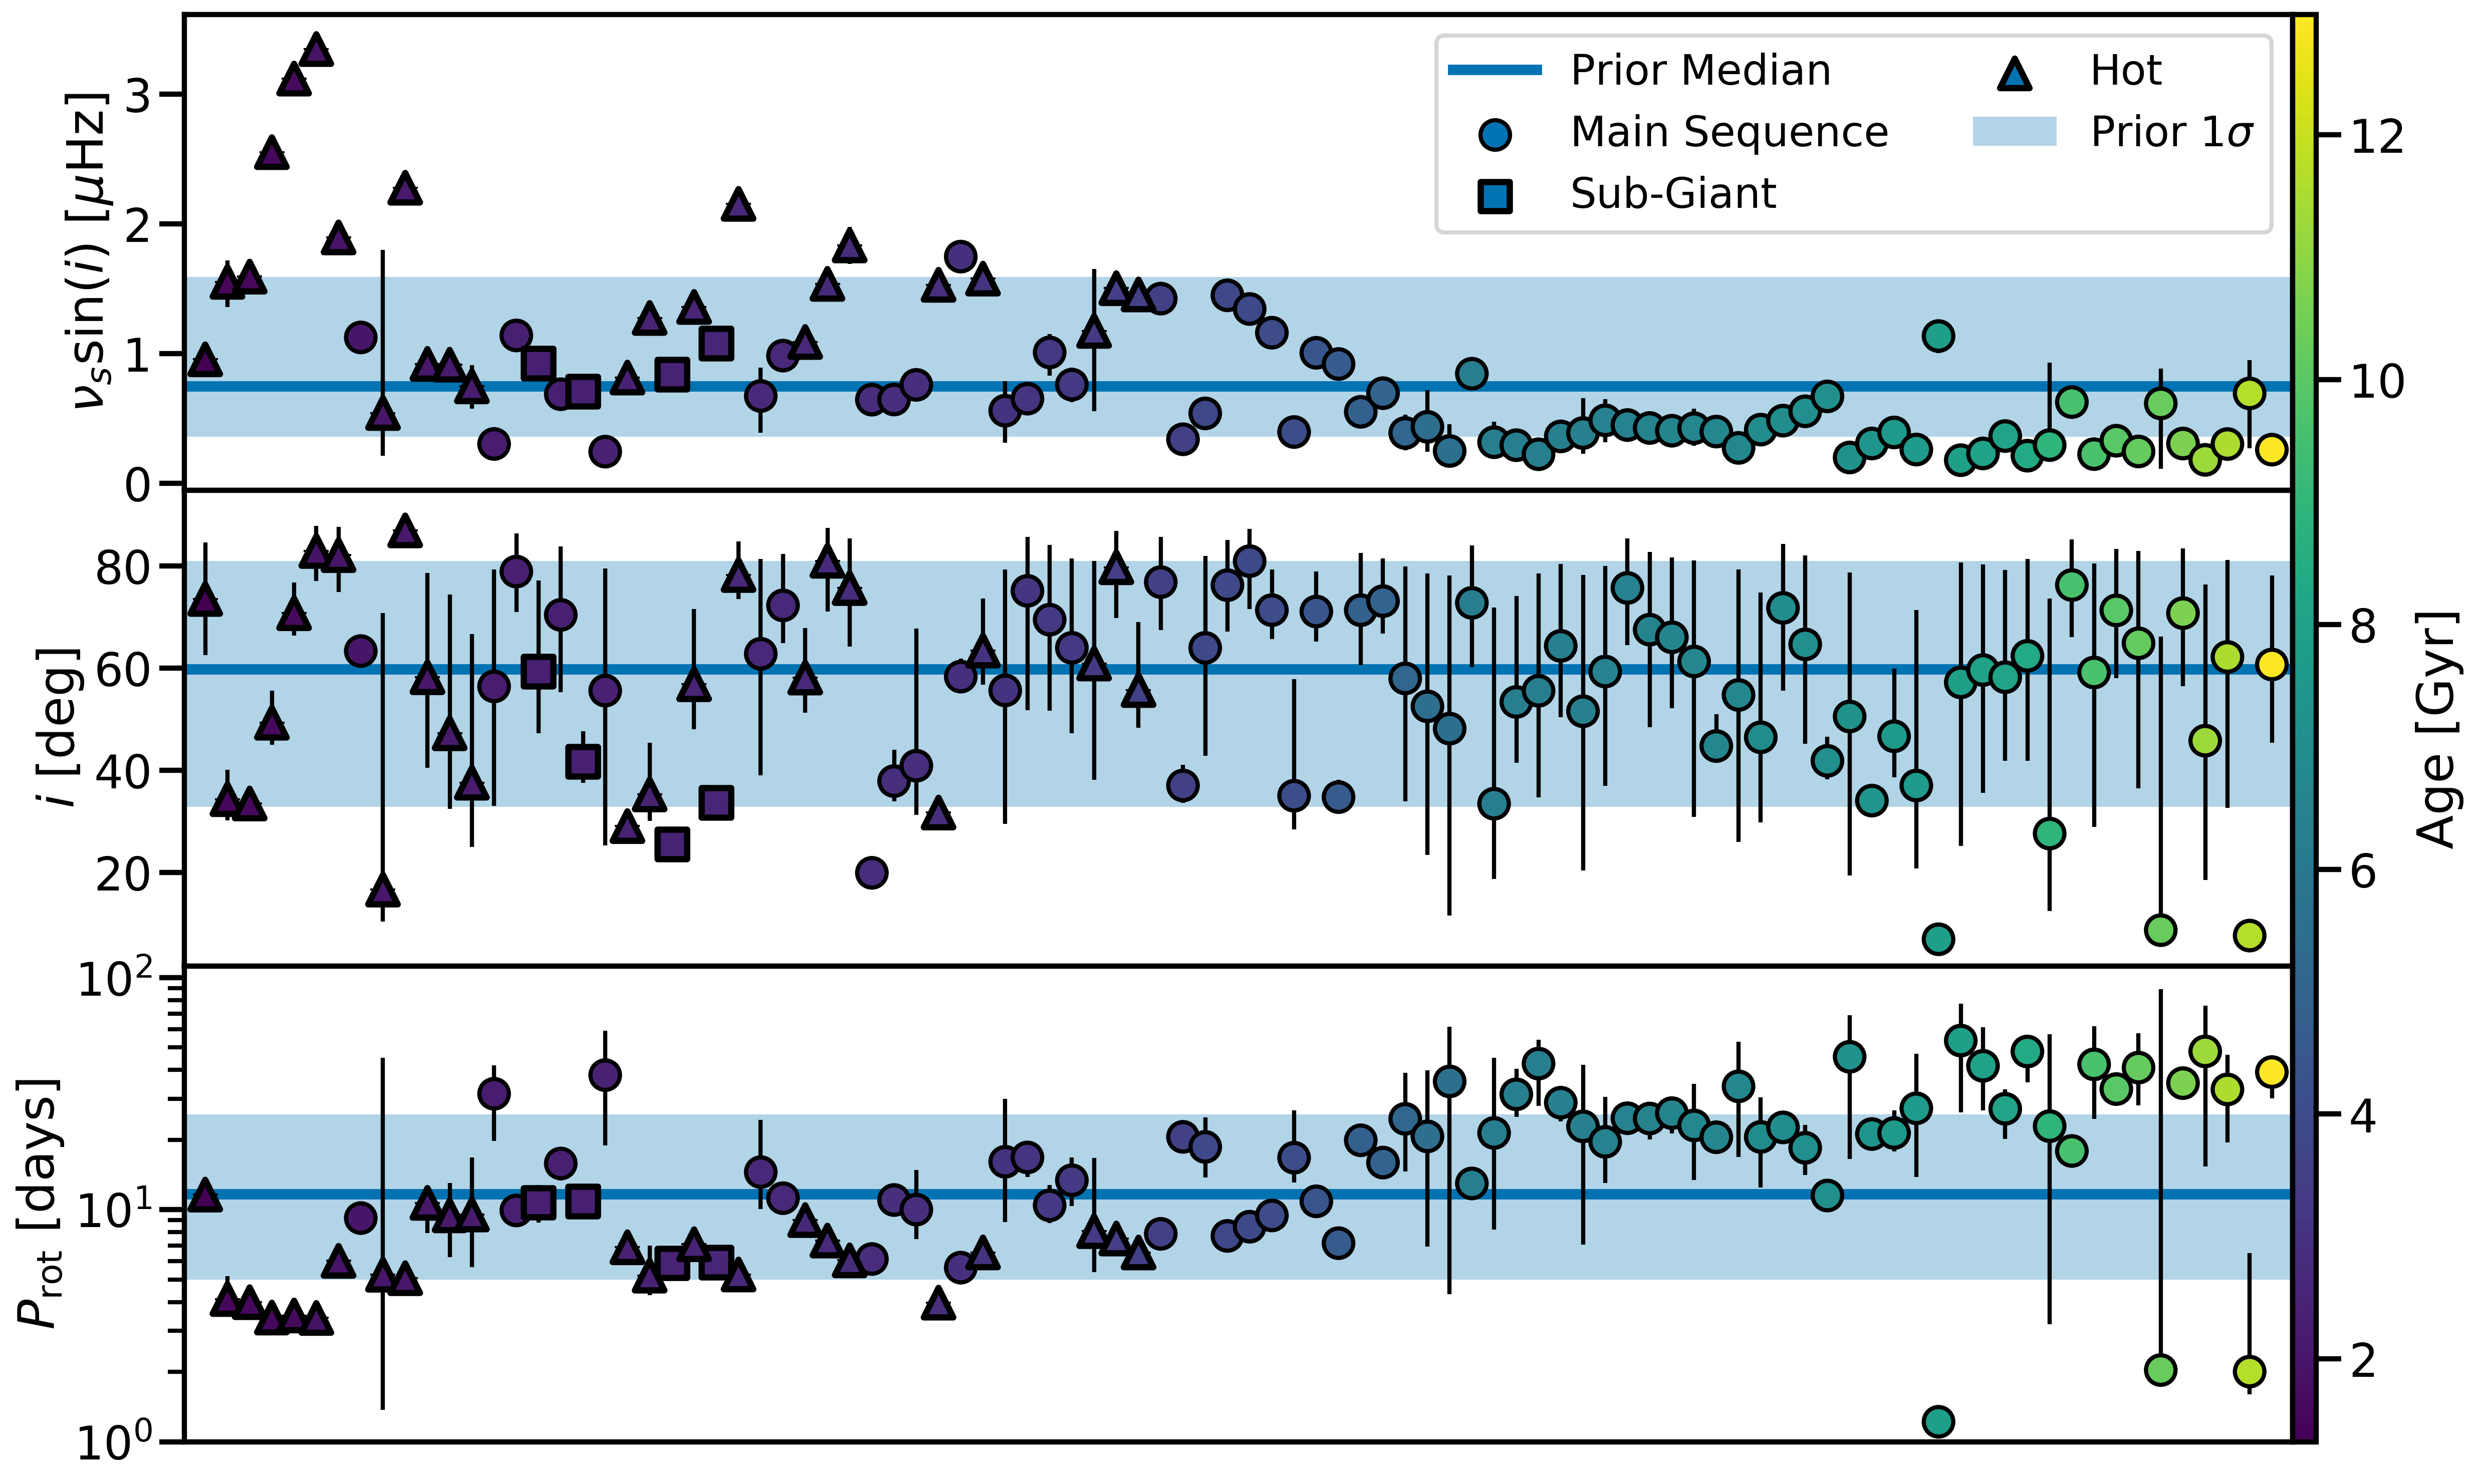
\includegraphics[width=\textwidth]{Images/priors.png}
	\caption{Comparisons between posterior estimates of rotational parameters (data points and error bars) and the priors on these parameters (shaded regions). Shown are projected splitting ($\nu_{\rm s}\sin(i)$), inclination angle ($i$, sampled as $\cos(i)$) and rotation period ($P$). Both the prior and values for $P$ are a transformation of the upper two parameters (see \textbf{Methods} and \textbf{Supplementary Information}) In all cases, the extent of the error bars and shaded regions indicate the 68\% credible ($1\sigma$) interval of the posterior and prior distributions respectively. The solid lines indicate the median of the prior distributions. In this figure, results with means and errorbars that closely resemble the prior distribution can be interpreted as prior-dominated (i.e. poorly informed by the data). All stars are sorted and coloured and sorted by age. In the case of inclination angle $i$ and rotation period $P$, the displayed priors are transformed from the priors imposed on the sampled parameters from which their posteriors were derived.}
	\label{fig:priors}
\end{figure}

\begin{figure*}[h!]
	\centering
	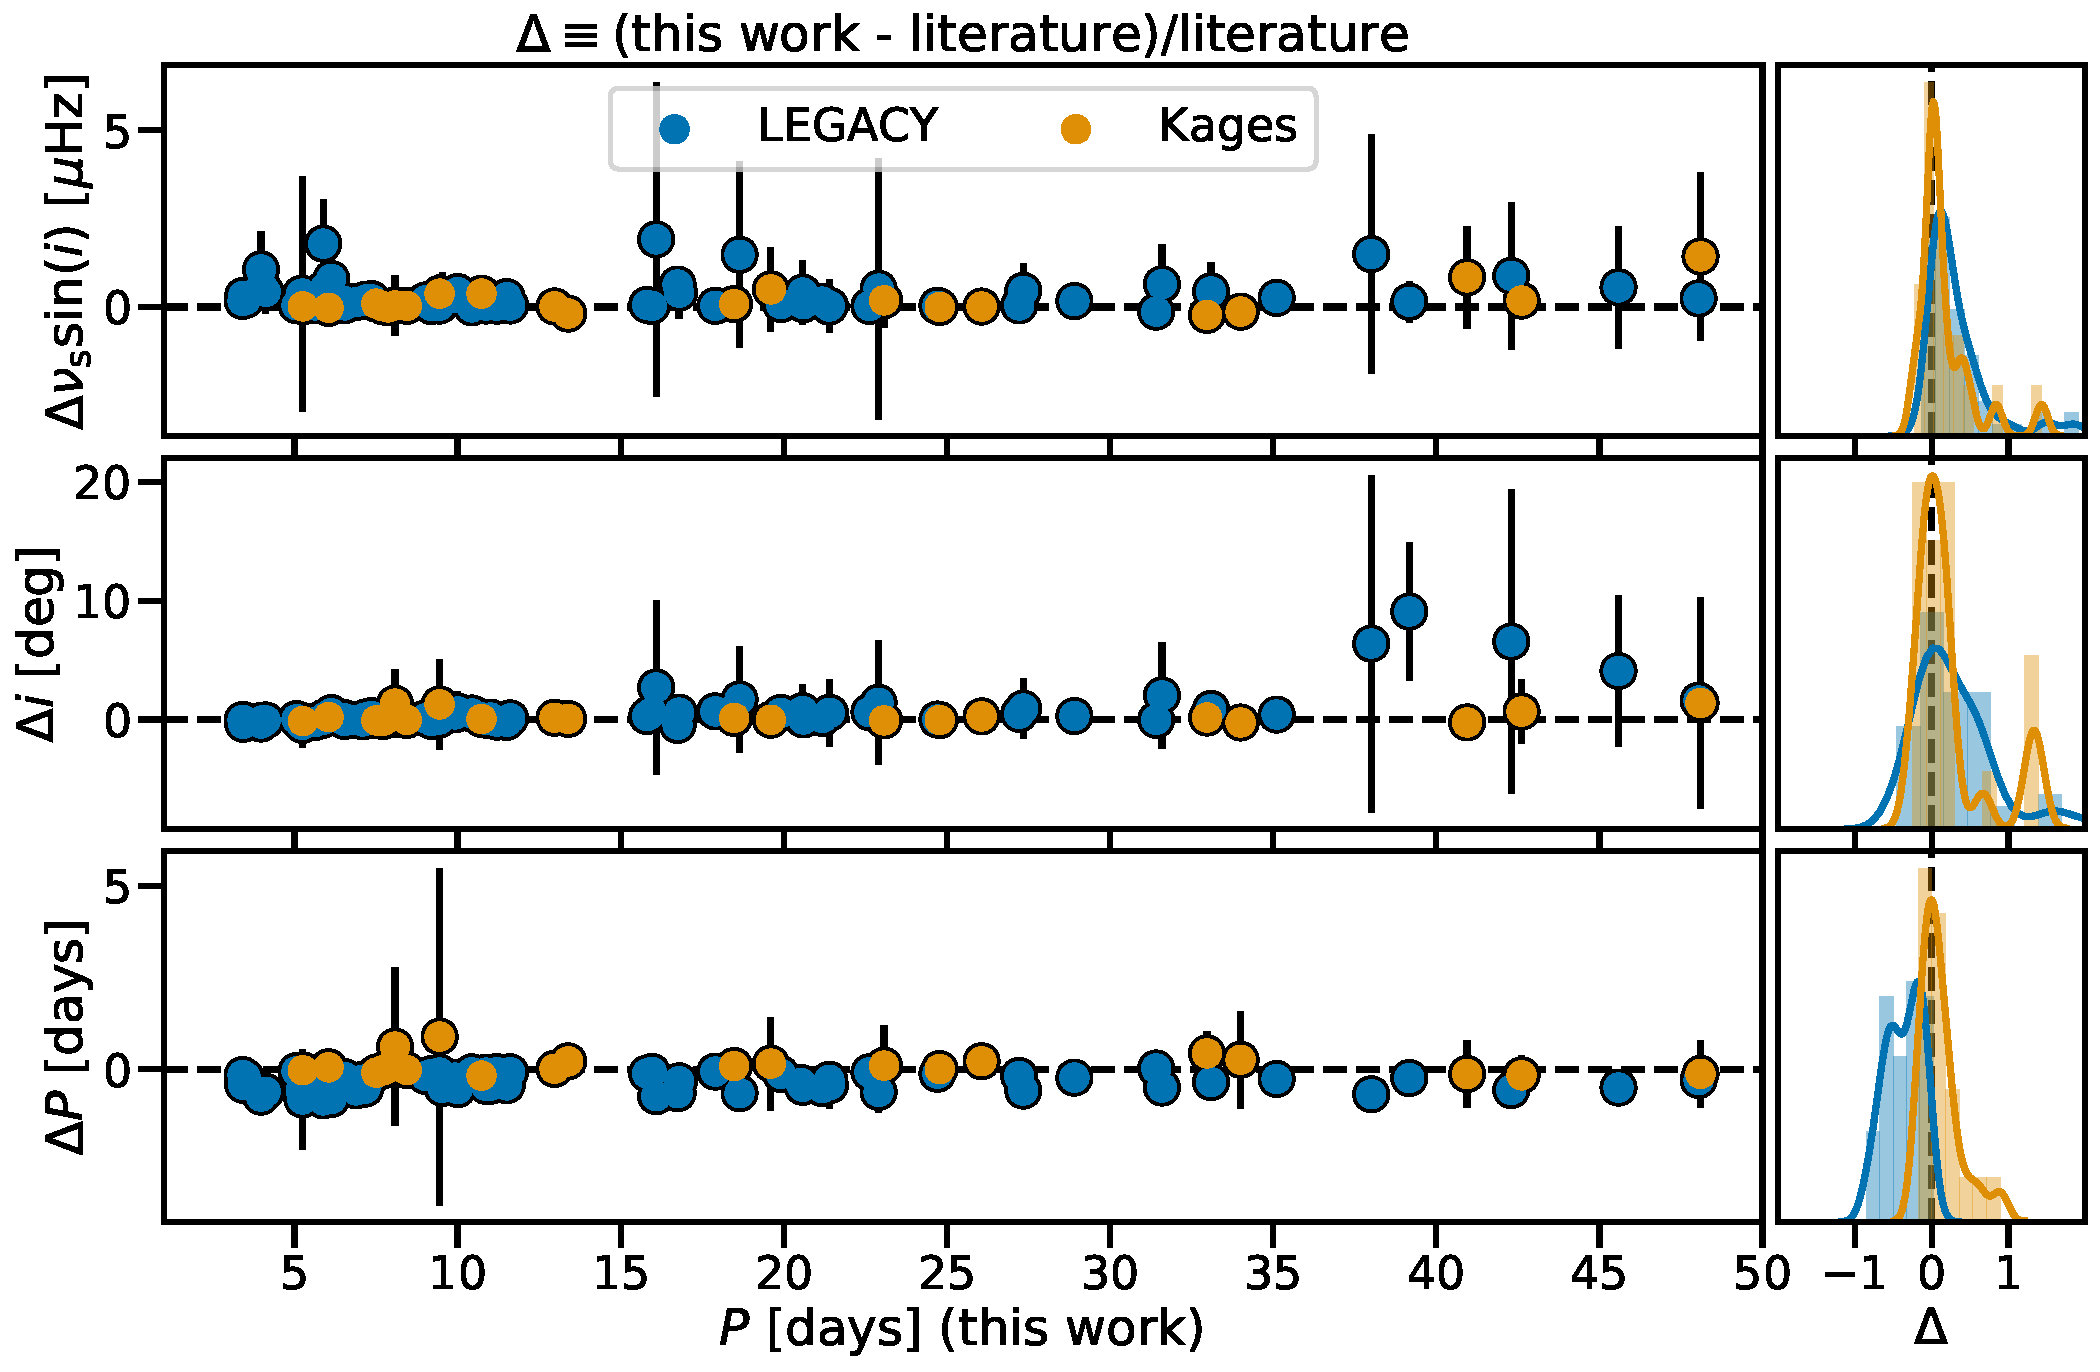
\includegraphics[width=\textwidth]{Images/litcomp_alt2.pdf}
	\caption{Comparisons between posterior estimates of rotational parameters from this work, LEGACY and `Kages' \cite[private communication]{m_davies+2016, m_lund+2017}.  Shown are projected splitting ($\nu_{\rm s}\sin(i)$), inclination angle ($i$, sampled as $\cos(i)$) and rotation period ($P$). Fractional differences are plotted against stellar rotation obtained in this work. The $\Delta$ indicates the fractional difference between this work and the literature (i.e. stars above the zero-line have higher values in this work). The right hand panels the distribution of the fractional differences around the zero line. The colour legend is consistent throughout all panels. The x-axis units on the right hand panels are equivalent to the y-axis of the left hand panels. 10 stars have been omitted from this plot and are discussed in more detail in \textbf{Methods}: KICs 5094751, 6196457, 8349582, 8494142, 8554498, 105114430 and 11133306 all have extremely low rotation periods in Kages, with high uncertainties. Conversely, KICs 6603624, 8760414 and 8938364 have extremely high rotation periods in LEGACY with low uncertainties. In cases where stars had asymmetric error bars, the larger of the two was used when propagating uncertainty for the purposes of this figure.}
	\label{fig:legacykages}
\end{figure*}
 
\begin{figure}[h!]
 \centering
 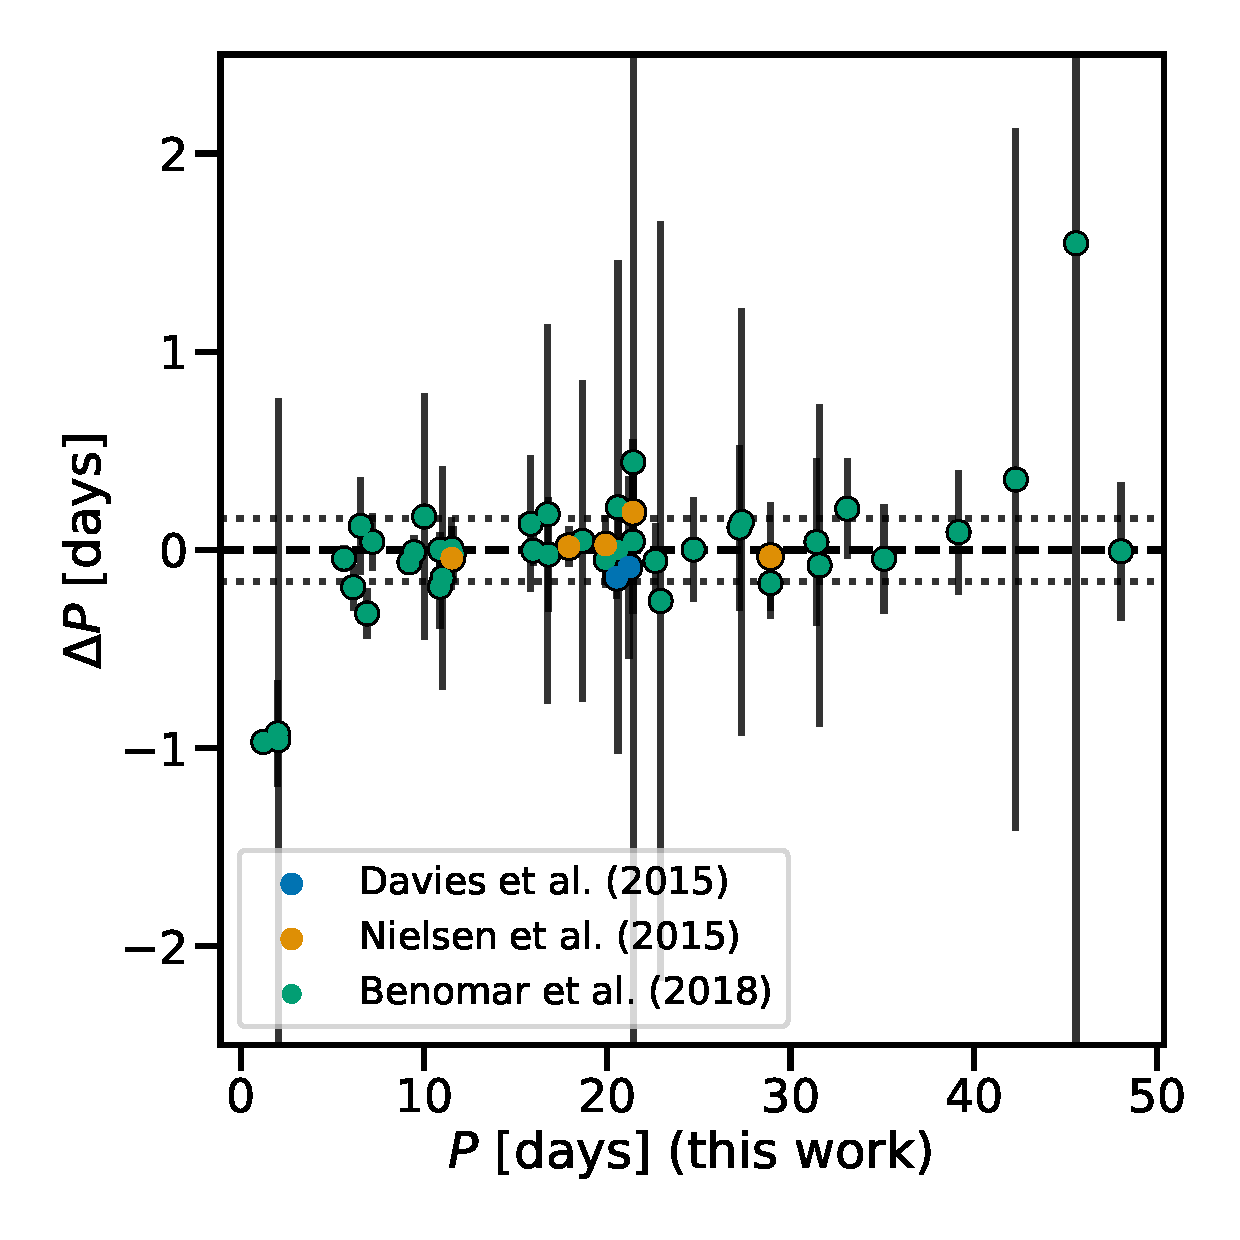
\includegraphics[width=0.8\textwidth]{Images/seis_comparison_rot_alt2.pdf}
 \caption{Fractional differences between posterior estimates of asteroseismic rotation period from this work. Literature sources are: Davies et al. (2015) \cite{m_davies+2015} (16 Cyg A \& B), Nielsen et al. (2015) \cite{m_nielsen+2015} (5 stars) and Benomar et al. (2018) \cite{m_benomar+2018} (40 stars). We used the reported parameter $a_{1}$ from the latter, which represents the rotational splitting in the case of uniform latitudinal rotation in their model. The dashed line represents the median of the sample shown, with the dotted lines representing the $15.9^{\rm{th}}$ and $84.1^{\rm{st}}$ percentiles. In cases where stars had asymmetric error bars, the larger of the two was used when propagating uncertainty for the purposes of this figure.}
 \label{fig:literaturecomp}
\end{figure}

 
 \begin{figure*}[h!]
 	\centering
 	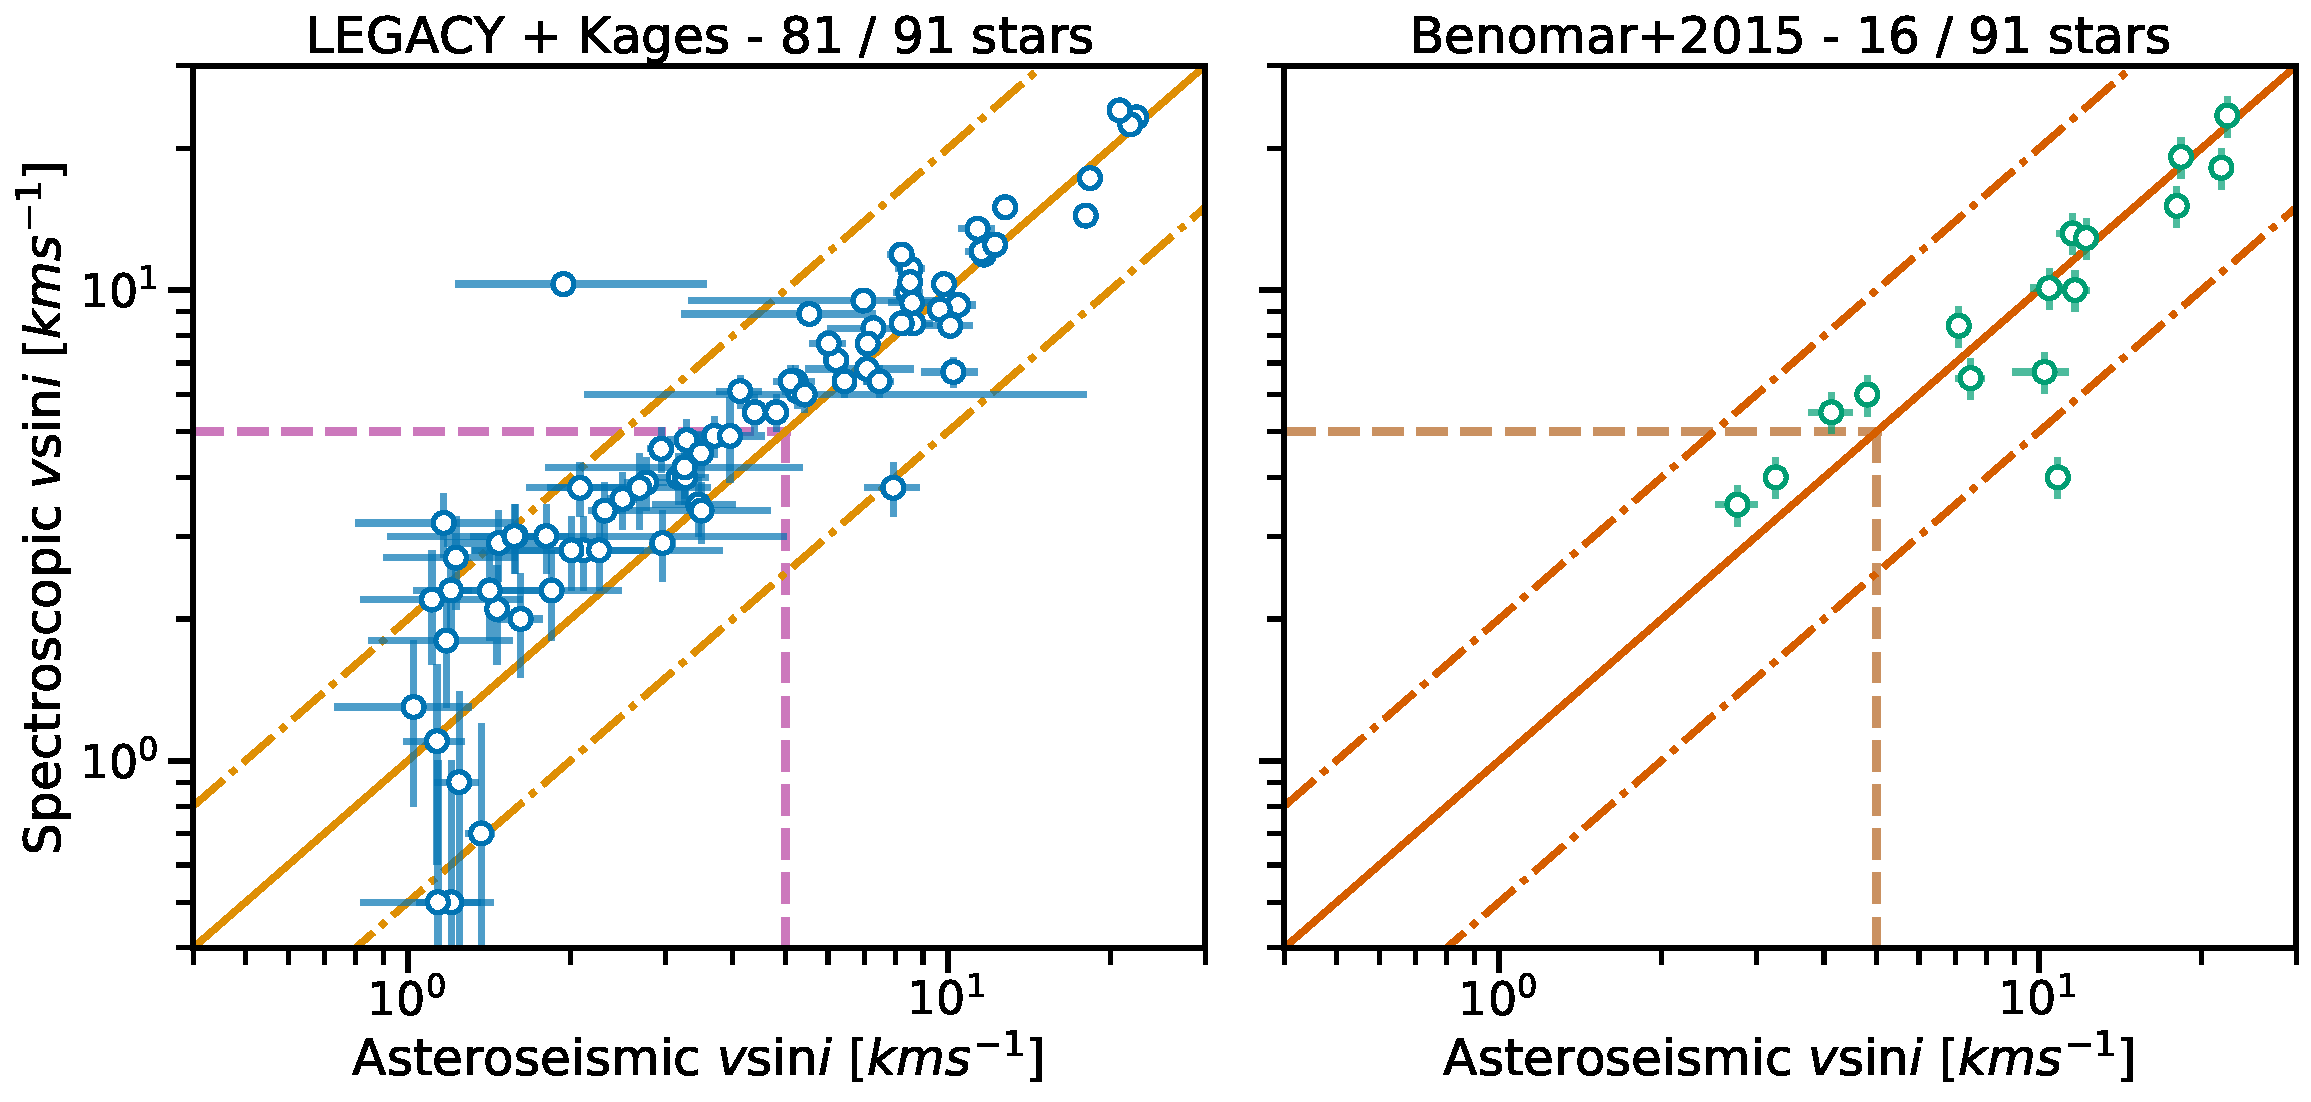
\includegraphics[width=\textwidth]{Images/vsini_comparison_new.pdf}
 	\caption{Comparisons between asteroseismic and spectroscopic measures of projected surface rotation, $\textrm{v}\sin(i)$. All asteroseismic (x-axis) values are from this work, all spectroscopic (y-axis) values are from the literature. \textit{Left}: comparisons to 81 stars values reported in LEGACY and Kages. \textit{Right}: comparisons to 16 stars observed by Benomar et al. (2015) \cite{m_benomar+2015}. Asteroseismic values are transformed from projected splitting ($\nu_s\sin(i)$) using the asteroseismic radius measurements presented in LEGACY and `Kages'. The solid lines indicate the 1:1 line, while the dash-dotted lines represent the 2:1 and 1:2 lines. The dashed lines indicate the location of $v\sin(i) = 5\, \rm{kms^{-1}}$, the point at which surface and seismic measures of projected rotation begin to differ strongly \cite{m_tayar+2015}.}
 	\label{fig:vsinilit}
 \end{figure*}

\begin{landscape}
\setlength\LTleft{0pt}
\setlength\LTright{0pt}
\footnotesize
\begin{longtable}{c|ccccc|ccc|ccc}
	\caption{Parameters for the 94 stars for which seismic rotation rates were obtained in this work. Temperature (\teff), age, mass, metallicity (\feh) and surface gravity ($\log(g)$) are adopted from the LEGACY \cite[L]{lund+2017,silvaaguirre+2017} and`Kages' \cite[K]{silvaaguirre+2015,davies+2016} catalogues, as listed in the Source column. Projected splitting ($\nu_{\rm s}\sin(i)$), inclination angle ($i$) and asteroseismic rotation ($P$) are from this work. Uncertainties were taken using the $15.9^{\rm th}$ and $84.1^{\rm st}$ percentiles of posterior distributions on the parameters, which are frequently asymmetrical in linear space. Reported values are the median of the posteriors. For parameters with no direct posterior samples (e.g. rotation) the full posterior samples were transformed before taking the summary statistics. The stellar type denotes whether a star is roughly classified as belonging to the main sequence (MS), Sub-Giants (SG) or `hot' stars (H) (see text).
		The flags indicate the following: 0; no issues, used in the gyrochronology analysis. 1; has either a number of effective samples $n_{\rm eff} < 1000$ for the asteroseismic splitting, or Gelman-Rubin convergence metric of $\hat{R} > 1.1$ \cite{gelman+rubin1992}, indicating that rotation measurements for these stars are less robust than those with a flag of 0. 2; was found to strongly disagree with multiple literature values, excluded from the gyrochronology analysis. 3; fell outside the model range of the stellar models, and were therefore not used in the gyrochronology analysis. Table is continued on the next page. A machine-readable version of the table is available (as Supplementary Data 1).}\label{tab:results}\\
	\toprule
	KIC & $T_{\rm{eff}}$ & Age & Mass & \feh & $\log(g)$ & $\nu_{\rm{s}}\sin(i)$ & $i$   & $P$   &  Flag & Type & Source \\
	& [$\mathrm{K}$] &  [$\mathrm{Gyr}$] & [$\mathrm{M_{\odot}}$] & [$\mathrm{dex}$] & [$\mathrm{dex}$] & [$\mathrm{\mu Hz}$]  & [$\mathrm{{}^{\circ}}$] & [$\mathrm{days}$]   &  &  &  \\
	\midrule
	\endfirsthead
	\caption[]{\textit{Continued from previous page.}}\\
	\toprule
	KIC & $T_{\rm{eff}}$ & Age & Mass & \feh & $\log(g)$ & $\nu_{\rm{s}}\sin(i)$ & $i$   & $P$   &  Flag & Type & Source \\
	& [$\mathrm{K}$] &  [$\mathrm{Gyr}$] & [$\mathrm{M_{\odot}}$] & [$\mathrm{dex}$] & [$\mathrm{dex}$] & [$\mathrm{\mu Hz}$]  & [$\mathrm{{}^{\circ}}$] & [$\mathrm{days}$]   &  &  &  \\
	\midrule
	\endhead
	\bottomrule \multicolumn{12}{r}{\textit{Continued on next page}}\\
	\endfoot
	\bottomrule
	\endlastfoot
	
	1435467 & 6326$\pm$77    & 3.02$_{-0.35}^{+0.50}$    & 1.32$_{-0.05}^{+0.03}$ & 0.01$\pm$0.10     & 4.100$_{-0.009}^{+0.009}$ & 1.58$_{-0.09}^{+0.10}$ & 63.4$_{-6.6}^{+10.2}$     & 6.5$_{-0.6}^{+0.8}$      & 0 &        H & L \\
	2837475 & 6614$\pm$77    & 1.63$_{-0.18}^{+0.11}$    & 1.43$_{-0.02}^{+0.02}$ & 0.01$\pm$0.10     & 4.163$_{-0.007}^{+0.007}$ & 3.12$_{-0.08}^{+0.08}$ & 70.7$_{-4.4}^{+6.0}$      & 3.5$_{-0.2}^{+0.2}$      & 0 &        H & L \\
	3425851 & 6343$\pm$85    & 3.32$_{-0.64}^{+0.85}$    & 1.18$_{-0.05}^{+0.05}$ & -0.04$\pm$0.10    & 4.243$_{-0.008}^{+0.008}$ & 1.17$_{-0.62}^{+0.48}$ & 60.9$_{-22.7}^{+20.1}$    & 8.1$_{-2.7}^{+8.6}$      & 0 &        H & K \\
	3427720 & 6045$\pm$77    & 2.23$_{-0.24}^{+0.24}$    & 1.11$_{-0.01}^{+0.02}$ & -0.06$\pm$0.10    & 4.387$_{-0.004}^{+0.005}$ & 0.30$_{-0.06}^{+0.06}$ & 56.4$_{-23.4}^{+22.9}$    & 31.6$_{-11.8}^{+10.2}$   & 0 &        MS & L \\
	3456181 & 6384$\pm$77    & 2.09$_{-0.13}^{+0.13}$    & 1.50$_{-0.02}^{+0.03}$ & -0.15$\pm$0.10    & 3.949$_{-0.009}^{+0.008}$ & 0.92$_{-0.08}^{+0.08}$ & 58.2$_{-17.7}^{+20.4}$    & 10.7$_{-2.8}^{+2.0}$     & 0 &        H & L \\
	3544595 & 5669$\pm$75    & 6.63$_{-0.57}^{+0.62}$    & 0.90$_{-0.01}^{+0.01}$ & -0.18$\pm$0.10    & 4.468$_{-0.003}^{+0.003}$ & 0.40$_{-0.04}^{+0.04}$ & 66.0$_{-13.9}^{+15.6}$    & 26.1$_{-4.7}^{+3.9}$     & 0 &        MS & K \\
	3632418 & 6193$\pm$77    & 2.63$_{-0.18}^{+0.18}$    & 1.41$_{-0.02}^{+0.02}$ & -0.12$\pm$0.10    & 4.024$_{-0.008}^{+0.008}$ & 0.98$_{-0.03}^{+0.03}$ & 72.3$_{-7.4}^{+10.0}$     & 11.2$_{-0.7}^{+0.6}$     & 0 &        MS & L \\
	3656476 & 5668$\pm$77    & 8.37$_{-1.57}^{+1.72}$    & 1.04$_{-0.04}^{+0.05}$ & 0.25$\pm$0.10     & 4.225$_{-0.010}^{+0.008}$ & 0.21$_{-0.02}^{+0.02}$ & 62.4$_{-20.5}^{+18.9}$    & 48.0$_{-12.7}^{+8.1}$    & 0 &        MS & L \\
	3735871 & 6107$\pm$77    & 2.35$_{-0.85}^{+1.04}$    & 1.09$_{-0.04}^{+0.04}$ & -0.04$\pm$0.10    & 4.396$_{-0.007}^{+0.007}$ & 0.69$_{-0.05}^{+0.05}$ & 70.4$_{-15.1}^{+13.4}$    & 15.8$_{-2.5}^{+1.8}$     & 0 &        MS & L \\
	4141376 & 6134$\pm$91    & 3.27$_{-0.64}^{+0.59}$    & 1.02$_{-0.03}^{+0.02}$ & -0.24$\pm$0.10    & 4.412$_{-0.003}^{+0.004}$ & 0.76$_{-0.13}^{+0.13}$ & 64.0$_{-16.7}^{+17.5}$    & 13.4$_{-3.0}^{+3.4}$     & 0 &        MS & K \\
	4143755 & 5622$\pm$106   & 11.27$_{-1.35}^{+1.50}$   & 0.92$_{-0.03}^{+0.02}$ & -0.40$\pm$0.11    & 4.102$_{-0.001}^{+0.002}$ & 0.18$_{-0.05}^{+0.08}$ & 45.8$_{-27.3}^{+30.6}$    & 48.1$_{-32.7}^{+27.4}$   & 1 &        MS & K \\
	4349452 & 6270$\pm$79    & 3.45$_{-0.72}^{+0.81}$    & 1.16$_{-0.05}^{+0.04}$ & -0.04$\pm$0.10    & 4.275$_{-0.007}^{+0.008}$ & 1.50$_{-0.09}^{+0.09}$ & 79.7$_{-10.0}^{+7.1}$      & 7.5$_{-0.6}^{+0.5}$     & 0 &        H & K \\
	4914423 & 5845$\pm$88    & 6.67$_{-0.62}^{+0.69}$    & 1.10$_{-0.03}^{+0.02}$ & 0.07$\pm$0.11     & 4.155$_{-0.004}^{+0.004}$ & 0.42$_{-0.14}^{+0.15}$ & 61.3$_{-30.5}^{+19.8}$    & 23.1$_{-9.6}^{+11.7}$    & 0 &        MS & K \\
	4914923 & 5805$\pm$77    & 7.57$_{-1.79}^{+1.66}$    & 1.06$_{-0.05}^{+0.06}$ & 0.08$\pm$0.10     & 4.197$_{-0.010}^{+0.008}$ & 0.39$_{-0.03}^{+0.03}$ & 46.6$_{-8.1}^{+13.3}$     & 21.4$_{-3.5}^{+5.4}$     & 0 &        MS & L \\
	5094751 & 5952$\pm$75    & 6.35$_{-1.05}^{+1.05}$    & 1.07$_{-0.04}^{+0.04}$ & -0.08$\pm$0.10    & 4.213$_{-0.008}^{+0.007}$ & 0.39$_{-0.16}^{+0.27}$ & 51.5$_{-31.1}^{+26.7}$    & 22.9$_{-15.8}^{+19.3}$   & 0 &        MS & K \\
	5184732 & 5846$\pm$77    & 4.85$_{-0.88}^{+1.57}$    & 1.15$_{-0.06}^{+0.04}$ & 0.36$\pm$0.10     & 4.255$_{-0.008}^{+0.010}$ & 0.55$_{-0.02}^{+0.02}$ & 71.3$_{-10.8}^{+11.2}$    & 19.9$_{-1.9}^{+1.3}$     & 0 &        MS & L \\
	5773345 & 6130$\pm$84    & 2.55$_{-0.24}^{+0.26}$    & 1.47$_{-0.03}^{+0.03}$ & 0.21$\pm$0.09     & 3.993$_{-0.007}^{+0.008}$ & 1.08$_{-0.08}^{+0.08}$ & 33.7$_{-2.5}^{+2.8}$      & 5.9$_{-0.5}^{+0.7}$      & 0 &        SG & L \\
	5866724 & 6169$\pm$50    & 3.89$_{-0.48}^{+0.59}$    & 1.20$_{-0.03}^{+0.03}$ & 0.09$\pm$0.08     & 4.224$_{-0.005}^{+0.007}$ & 1.34$_{-0.08}^{+0.07}$ & 80.9$_{-9.4}^{+6.3}$      & 8.4$_{-0.5}^{+0.5}$      & 0 &        MS & K \\
	5950854 & 5853$\pm$77    & 8.93$_{-1.15}^{+1.12}$    & 0.97$_{-0.03}^{+0.03}$ & -0.23$\pm$0.10    & 4.238$_{-0.007}^{+0.007}$ & 0.29$_{-0.12}^{+0.64}$ & 27.6$_{-15.2}^{+46.0}$    & 22.9$_{-19.7}^{+34.2}$   & 1 &        MS & L \\
	6106415 & 6037$\pm$77    & 5.03$_{-1.12}^{+1.28}$    & 1.07$_{-0.04}^{+0.05}$ & -0.04$\pm$0.10    & 4.295$_{-0.009}^{+0.009}$ & 0.69$_{-0.02}^{+0.02}$ & 73.1$_{-6.3}^{+8.4}$      & 16.0$_{-0.8}^{+0.7}$     & 0 &        MS & L \\
	6116048 & 6033$\pm$77    & 9.58$_{-1.90}^{+2.16}$    & 0.94$_{-0.05}^{+0.05}$ & -0.23$\pm$0.10    & 4.254$_{-0.012}^{+0.009}$ & 0.63$_{-0.02}^{+0.02}$ & 76.3$_{-10.2}^{+9.0}$     & 17.9$_{-1.2}^{+0.8}$     & 0 &        MS & L \\
	6196457 & 5871$\pm$94    & 5.52$_{-0.48}^{+0.51}$    & 1.21$_{-0.03}^{+0.02}$ & 0.17$\pm$0.11     & 4.049$_{-0.004}^{+0.005}$ & 0.43$_{-0.19}^{+0.28}$ & 52.5$_{-29.1}^{+26.0}$    & 20.7$_{-13.7}^{+19.2}$   & 0 &        MS & K \\
	6225718 & 6313$\pm$76    & 2.41$_{-0.43}^{+0.53}$    & 1.16$_{-0.03}^{+0.03}$ & -0.07$\pm$0.10    & 4.319$_{-0.007}^{+0.005}$ & 0.81$_{-0.03}^{+0.03}$ & 29.1$_{-1.8}^{+2.1}$      & 6.9$_{-0.5}^{+0.6}$      & 0 &        H & L \\
	6278762 & 5046$\pm$74    & 11.54$_{-0.94}^{+0.99}$   & 0.74$_{-0.01}^{+0.01}$ & -0.37$\pm$0.09    & 4.560$_{-0.003}^{+0.002}$ & 0.30$_{-0.09}^{+0.09}$ & 62.2$_{-29.5}^{+19.0}$    & 33.0$_{-13.5}^{+13.6}$   & 1, 3 &        MS & K \\
	6508366 & 6331$\pm$77    & 2.06$_{-0.14}^{+0.13}$    & 1.53$_{-0.02}^{+0.03}$ & -0.05$\pm$0.10    & 3.942$_{-0.007}^{+0.005}$ & 2.28$_{-0.04}^{+0.04}$ & 87.0$_{-3.2}^{+2.1}$      & 5.1$_{-0.1}^{+0.1}$      & 0 &        H & L \\
	6521045 & 5825$\pm$75    & 6.50$_{-0.56}^{+0.46}$    & 1.11$_{-0.02}^{+0.02}$ & 0.02$\pm$0.10     & 4.125$_{-0.004}^{+0.004}$ & 0.45$_{-0.02}^{+0.03}$ & 75.7$_{-11.2}^{+9.7}$     & 24.8$_{-2.0}^{+1.9}$     & 0 &        MS & K \\
	6603624 & 5674$\pm$77    & 7.82$_{-0.86}^{+0.94}$    & 1.01$_{-0.02}^{+0.03}$ & 0.28$\pm$0.10     & 4.320$_{-0.005}^{+0.004}$ & 1.13$_{-0.13}^{+0.13}$ & 6.9$_{-0.8}^{+0.8}$       & 1.2$_{-0.0}^{+0.0}$      & 2 &        MS & L \\
	6679371 & 6479$\pm$77    & 1.95$_{-0.16}^{+0.18}$    & 1.53$_{-0.02}^{+0.04}$ & 0.01$\pm$0.10     & 3.934$_{-0.008}^{+0.007}$ & 1.90$_{-0.06}^{+0.05}$ & 82.1$_{-7.2}^{+5.5}$      & 6.0$_{-0.2}^{+0.2}$      & 0 &        H & L \\
	6933899 & 5832$\pm$77    & 6.34$_{-0.62}^{+0.72}$    & 1.13$_{-0.03}^{+0.03}$ & -0.01$\pm$0.10    & 4.087$_{-0.007}^{+0.008}$ & 0.36$_{-0.02}^{+0.02}$ & 64.3$_{-14.0}^{+16.1}$    & 28.9$_{-4.8}^{+3.7}$     & 0 &        MS & L \\
	7103006 & 6344$\pm$77    & 2.47$_{-0.24}^{+0.22}$    & 1.42$_{-0.02}^{+0.04}$ & 0.02$\pm$0.10     & 4.015$_{-0.007}^{+0.007}$ & 1.36$_{-0.09}^{+0.08}$ & 56.8$_{-8.8}^{+14.8}$     & 7.1$_{-1.0}^{+1.3}$      & 0 &        H & L \\
	7106245 & 6068$\pm$102   & 6.27$_{-1.06}^{+1.06}$    & 0.92$_{-0.04}^{+0.02}$ & -0.99$\pm$0.19    & 4.325$_{-0.007}^{+0.007}$ & 0.32$_{-0.10}^{+0.16}$ & 33.4$_{-14.7}^{+38.4}$    & 21.4$_{-13.2}^{+23.8}$   & 1, 3 &        MS & L \\
	7206837 & 6305$\pm$77    & 2.90$_{-0.30}^{+0.42}$    & 1.30$_{-0.03}^{+0.03}$ & 0.10$\pm$0.10     & 4.163$_{-0.007}^{+0.008}$ & 1.53$_{-0.12}^{+0.12}$ & 31.7$_{-2.8}^{+3.2}$      & 4.0$_{-0.4}^{+0.6}$      & 0 &        H & L \\
	7296438 & 5775$\pm$77    & 7.23$_{-1.77}^{+1.49}$    & 1.08$_{-0.05}^{+0.06}$ & 0.19$\pm$0.10     & 4.201$_{-0.010}^{+0.009}$ & 0.20$_{-0.06}^{+0.06}$ & 50.5$_{-31.1}^{+28.2}$    & 45.6$_{-29.0}^{+23.4}$   & 1 &        MS & L \\
	7510397 & 6171$\pm$77    & 2.82$_{-0.16}^{+0.14}$    & 1.37$_{-0.02}^{+0.02}$ & -0.21$\pm$0.10    & 4.036$_{-0.004}^{+0.007}$ & 0.64$_{-0.06}^{+0.06}$ & 19.9$_{-2.0}^{+2.0}$      & 6.1$_{-0.6}^{+0.7}$      & 0 &        MS & L \\
	7670943 & 6463$\pm$110   & 2.78$_{-0.51}^{+0.62}$    & 1.24$_{-0.05}^{+0.04}$ & 0.09$\pm$0.11     & 4.228$_{-0.008}^{+0.008}$ & 1.83$_{-0.14}^{+0.14}$ & 75.7$_{-11.5}^{+9.8}$     & 6.0$_{-0.6}^{+0.6}$      & 0 &        H & K \\
	7680114 & 5811$\pm$77    & 7.68$_{-1.28}^{+1.45}$    & 1.06$_{-0.05}^{+0.04}$ & 0.05$\pm$0.10     & 4.172$_{-0.010}^{+0.008}$ & 0.26$_{-0.04}^{+0.05}$ & 37.0$_{-16.3}^{+34.3}$    & 27.3$_{-13.5}^{+19.6}$   & 0 &        MS & L \\
	7771282 & 6248$\pm$77    & 3.24$_{-0.32}^{+0.35}$    & 1.29$_{-0.03}^{+0.03}$ & -0.02$\pm$0.10    & 4.112$_{-0.007}^{+0.007}$ & 1.01$_{-0.18}^{+0.14}$ & 69.5$_{-17.8}^{+14.6}$    & 10.4$_{-1.7}^{+2.3}$     & 0 &        MS & L \\
	7871531 & 5501$\pm$77    & 9.96$_{-1.77}^{+1.93}$    & 0.83$_{-0.02}^{+0.03}$ & -0.26$\pm$0.10    & 4.478$_{-0.005}^{+0.007}$ & 0.33$_{-0.03}^{+0.03}$ & 71.3$_{-13.2}^{+12.0}$    & 33.1$_{-4.1}^{+4.1}$     & 0 &        MS & L \\
	7940546 & 6235$\pm$77    & 2.33$_{-0.08}^{+0.08}$    & 1.40$_{-0.01}^{+0.03}$ & -0.20$\pm$0.10    & 4.007$_{-0.001}^{+0.003}$ & 1.14$_{-0.03}^{+0.03}$ & 78.9$_{-7.9}^{+7.4}$      & 9.9$_{-0.4}^{+0.3}$      & 0 &        MS & L \\
	7970740 & 5309$\pm$77    & 12.98$_{-2.00}^{+1.36}$   & 0.73$_{-0.01}^{+0.03}$ & -0.54$\pm$0.10    & 4.539$_{-0.005}^{+0.004}$ & 0.26$_{-0.02}^{+0.03}$ & 60.7$_{-15.3}^{+17.4}$    & 39.2$_{-9.0}^{+6.7}$     & 0 &        MS & L \\
	8006161 & 5488$\pm$77    & 3.59$_{-1.45}^{+1.53}$    & 0.98$_{-0.03}^{+0.03}$ & 0.34$\pm$0.10     & 4.494$_{-0.007}^{+0.007}$ & 0.34$_{-0.02}^{+0.02}$ & 37.0$_{-3.4}^{+4.1}$      & 20.6$_{-1.8}^{+2.2}$     & 0 &        MS & L \\
	8077137 & 6072$\pm$75    & 6.23$_{-1.23}^{+0.56}$    & 1.12$_{-0.05}^{+0.04}$ & -0.09$\pm$0.10    & 4.056$_{-0.013}^{+0.010}$ & 0.84$_{-0.07}^{+0.06}$ & 72.8$_{-12.6}^{+11.3}$    & 13.0$_{-1.5}^{+1.3}$     & 0 &        MS & K \\
	8150065 & 6173$\pm$101   & 3.83$_{-0.67}^{+0.99}$    & 1.19$_{-0.05}^{+0.04}$ & -0.13$\pm$0.15    & 4.220$_{-0.008}^{+0.008}$ & 0.54$_{-0.13}^{+0.11}$ & 64.0$_{-21.1}^{+18.0}$    & 18.6$_{-4.9}^{+6.4}$     & 0 &        MS & L \\
	8179536 & 6343$\pm$77    & 3.54$_{-0.81}^{+1.04}$    & 1.16$_{-0.06}^{+0.05}$ & -0.03$\pm$0.10    & 4.255$_{-0.010}^{+0.010}$ & 1.46$_{-0.09}^{+0.10}$ & 55.7$_{-7.4}^{+13.3}$     & 6.5$_{-0.8}^{+1.2}$      & 0 &        H & L \\
	8228742 & 6122$\pm$77    & 2.89$_{-0.18}^{+0.16}$    & 1.38$_{-0.02}^{+0.02}$ & -0.08$\pm$0.10    & 4.035$_{-0.005}^{+0.007}$ & 0.64$_{-0.04}^{+0.04}$ & 37.9$_{-4.0}^{+6.2}$      & 11.0$_{-1.3}^{+2.0}$     & 0 &        MS & L \\
	8292840 & 6239$\pm$94    & 3.85$_{-0.75}^{+0.81}$    & 1.15$_{-0.05}^{+0.05}$ & -0.14$\pm$0.10    & 4.240$_{-0.008}^{+0.008}$ & 1.45$_{-0.07}^{+0.07}$ & 76.2$_{-9.1}^{+8.9}$      & 7.7$_{-0.5}^{+0.5}$      & 0 &        MS & K \\
	8349582 & 5699$\pm$74    & 8.03$_{-0.70}^{+0.80}$    & 1.07$_{-0.02}^{+0.02}$ & 0.30$\pm$0.10     & 4.163$_{-0.003}^{+0.004}$ & 0.23$_{-0.06}^{+0.07}$ & 59.6$_{-24.1}^{+20.7}$    & 41.7$_{-14.9}^{+19.6}$   & 1 &        MS & K \\
	8379927 & 6067$\pm$120   & 1.99$_{-0.75}^{+0.85}$    & 1.12$_{-0.04}^{+0.04}$ & -0.10$\pm$0.15    & 4.388$_{-0.007}^{+0.008}$ & 1.12$_{-0.02}^{+0.02}$ & 63.3$_{-2.3}^{+2.5}$      & 9.2$_{-0.2}^{+0.3}$      & 0 &        MS & L \\
	8394589 & 6143$\pm$77    & 4.45$_{-0.83}^{+0.94}$    & 1.04$_{-0.03}^{+0.04}$ & -0.29$\pm$0.10    & 4.322$_{-0.008}^{+0.008}$ & 1.01$_{-0.03}^{+0.03}$ & 71.1$_{-5.9}^{+7.9}$      & 10.9$_{-0.6}^{+0.6}$     & 0 &        MS & L \\
	8424992 & 5719$\pm$77    & 9.61$_{-1.74}^{+1.92}$    & 0.92$_{-0.04}^{+0.04}$ & -0.12$\pm$0.10    & 4.359$_{-0.007}^{+0.007}$ & 0.22$_{-0.06}^{+0.06}$ & 59.1$_{-30.3}^{+21.3}$    & 42.3$_{-17.7}^{+19.4}$   & 1 &        MS & L \\
	8494142 & 6144$\pm$106   & 2.62$_{-0.24}^{+0.26}$    & 1.42$_{-0.02}^{+0.03}$ & 0.13$\pm$0.10     & 4.038$_{-0.005}^{+0.005}$ & 0.67$_{-0.28}^{+0.22}$ & 62.8$_{-23.8}^{+18.5}$    & 14.5$_{-4.5}^{+9.9}$     & 0 &        MS & K \\
	8554498 & 5945$\pm$60    & 5.60$_{-0.42}^{+0.45}$    & 1.20$_{-0.03}^{+0.02}$ & 0.17$\pm$0.05     & 4.007$_{-0.003}^{+0.003}$ & 0.25$_{-0.09}^{+0.21}$ & 48.1$_{-36.6}^{+30.0}$    & 35.7$_{-31.4}^{+25.6}$   & 0 &        MS & K \\
	8694723 & 6246$\pm$77    & 4.69$_{-0.51}^{+0.48}$    & 1.14$_{-0.02}^{+0.02}$ & -0.42$\pm$0.10    & 4.113$_{-0.009}^{+0.007}$ & 0.92$_{-0.05}^{+0.05}$ & 34.7$_{-2.7}^{+3.4}$      & 7.2$_{-0.6}^{+0.8}$      & 0 &        MS & L \\
	8760414 & 5873$\pm$77    & 11.66$_{-1.61}^{+1.28}$   & 0.81$_{-0.02}^{+0.03}$ & -0.92$\pm$0.10    & 4.329$_{-0.005}^{+0.006}$ & 0.69$_{-0.42}^{+0.26}$ & 7.6$_{-1.7}^{+2.3}$       & 2.0$_{-0.4}^{+4.5}$      & 2, 3 &        MS & L \\
	8866102 & 6325$\pm$75    & 2.60$_{-0.53}^{+0.56}$    & 1.23$_{-0.04}^{+0.04}$ & 0.01$\pm$0.10     & 4.262$_{-0.007}^{+0.008}$ & 2.15$_{-0.04}^{+0.04}$ & 78.2$_{-4.7}^{+6.6}$      & 5.3$_{-0.2}^{+0.2}$      & 0 &        H & K \\
	8938364 & 5677$\pm$77    & 10.25$_{-0.65}^{+0.56}$   & 0.99$_{-0.01}^{+0.01}$ & -0.13$\pm$0.10    & 4.173$_{-0.002}^{+0.007}$ & 0.61$_{-0.50}^{+0.27}$ & 8.7$_{-2.3}^{+57.5}$      & 2.0$_{-0.2}^{+87.0}$     & 2 &        MS & L \\
	9025370 & 5270$\pm$180   & 6.55$_{-1.13}^{+1.26}$    & 0.97$_{-0.03}^{+0.03}$ & -0.12$\pm$0.18    & 4.423$_{-0.004}^{+0.007}$ & 0.43$_{-0.04}^{+0.04}$ & 67.5$_{-19.1}^{+15.2}$    & 24.7$_{-4.7}^{+3.7}$     & 0 &        MS & L \\
	9098294 & 5852$\pm$77    & 8.08$_{-0.73}^{+0.99}$    & 0.97$_{-0.03}^{+0.02}$ & -0.18$\pm$0.10    & 4.308$_{-0.007}^{+0.005}$ & 0.36$_{-0.04}^{+0.04}$ & 58.2$_{-16.3}^{+21.0}$    & 27.2$_{-7.0}^{+5.7}$     & 0 &        MS & L \\
	9139151 & 6302$\pm$77    & 1.32$_{-0.75}^{+0.94}$    & 1.18$_{-0.05}^{+0.04}$ & 0.10$\pm$0.10     & 4.382$_{-0.008}^{+0.008}$ & 0.95$_{-0.04}^{+0.04}$ & 73.5$_{-11.0}^{+11.0}$    & 11.6$_{-1.1}^{+0.8}$     & 0 &        H & L \\
	9139163 & 6400$\pm$84    & 1.60$_{-0.22}^{+0.22}$    & 1.40$_{-0.02}^{+0.03}$ & 0.15$\pm$0.09     & 4.200$_{-0.008}^{+0.009}$ & 1.59$_{-0.08}^{+0.07}$ & 33.5$_{-3.0}^{+3.0}$      & 4.0$_{-0.3}^{+0.3}$      & 1 &        H & L \\
	9206432 & 6538$\pm$77    & 1.53$_{-0.30}^{+0.21}$    & 1.38$_{-0.02}^{+0.04}$ & 0.16$\pm$0.10     & 4.220$_{-0.007}^{+0.005}$ & 1.55$_{-0.20}^{+0.17}$ & 34.3$_{-4.2}^{+5.7}$      & 4.1$_{-0.5}^{+1.0}$      & 0 &        H & L \\
	9353712 & 6278$\pm$77    & 2.15$_{-0.13}^{+0.11}$    & 1.51$_{-0.02}^{+0.03}$ & -0.05$\pm$0.10    & 3.943$_{-0.005}^{+0.007}$ & 0.75$_{-0.17}^{+0.16}$ & 37.6$_{-12.6}^{+29.1}$    & 9.5$_{-3.9}^{+7.3}$      & 0 &        H & L \\
	9410862 & 6047$\pm$77    & 6.93$_{-1.33}^{+1.49}$    & 0.97$_{-0.04}^{+0.05}$ & -0.31$\pm$0.10    & 4.300$_{-0.008}^{+0.009}$ & 0.41$_{-0.08}^{+0.09}$ & 46.4$_{-16.7}^{+28.3}$    & 20.6$_{-8.1}^{+9.8}$     & 1 &        MS & L \\
	9414417 & 6253$\pm$75    & 2.65$_{-0.18}^{+0.16}$    & 1.40$_{-0.03}^{+0.02}$ & -0.13$\pm$0.10    & 4.016$_{-0.005}^{+0.005}$ & 1.09$_{-0.05}^{+0.05}$ & 58.1$_{-6.9}^{+9.7}$      & 9.0$_{-0.9}^{+1.1}$      & 0 &        H & L \\
	9592705 & 6174$\pm$92    & 2.33$_{-0.16}^{+0.18}$    & 1.51$_{-0.02}^{+0.03}$ & 0.22$\pm$0.10     & 3.961$_{-0.004}^{+0.003}$ & 0.93$_{-0.09}^{+0.09}$ & 59.3$_{-12.1}^{+17.8}$    & 10.7$_{-1.9}^{+2.1}$     & 0 &        SG & K \\
	9812850 & 6321$\pm$77    & 2.71$_{-0.35}^{+0.46}$    & 1.37$_{-0.05}^{+0.04}$ & -0.07$\pm$0.10    & 4.053$_{-0.009}^{+0.008}$ & 1.54$_{-0.08}^{+0.09}$ & 81.0$_{-10.0}^{+6.4}$      & 7.4$_{-0.5}^{+0.4}$     & 0 &        H & L \\
	9955598 & 5457$\pm$77    & 6.29$_{-1.84}^{+1.95}$    & 0.90$_{-0.03}^{+0.04}$ & 0.05$\pm$0.10     & 4.497$_{-0.005}^{+0.007}$ & 0.29$_{-0.04}^{+0.04}$ & 53.4$_{-11.9}^{+20.8}$    & 31.4$_{-6.4}^{+9.1}$     & 0 &        MS & L \\
	9965715 & 5860$\pm$180   & 2.92$_{-0.75}^{+0.86}$    & 1.21$_{-0.05}^{+0.04}$ & -0.44$\pm$0.18    & 4.272$_{-0.009}^{+0.008}$ & 1.75$_{-0.05}^{+0.05}$ & 58.3$_{-3.2}^{+3.5}$      & 5.6$_{-0.3}^{+0.3}$      & 0 &        MS & L \\
	10068307 & 6132$\pm$77   & 2.36$_{-0.10}^{+0.08}$    & 1.47$_{-0.02}^{+0.01}$ & -0.23$\pm$0.10    & 3.967$_{-0.004}^{+0.004}$ & 0.71$_{-0.03}^{+0.03}$ & 41.7$_{-4.1}^{+6.0}$      & 10.9$_{-1.1}^{+1.5}$     & 0 &        SG & L \\
	10079226 & 5949$\pm$77   & 3.06$_{-0.65}^{+0.70}$    & 1.12$_{-0.03}^{+0.02}$ & 0.11$\pm$0.10     & 4.366$_{-0.005}^{+0.005}$ & 0.65$_{-0.08}^{+0.07}$ & 75.1$_{-23.4}^{+10.6}$    & 16.8$_{-3.0}^{+2.2}$     & 1 &        MS & L \\
	10162436 & 6146$\pm$77   & 2.46$_{-0.11}^{+0.10}$    & 1.45$_{-0.01}^{+0.02}$ & -0.16$\pm$0.10    & 3.981$_{-0.005}^{+0.005}$ & 0.84$_{-0.05}^{+0.05}$ & 25.5$_{-1.8}^{+2.1}$      & 5.9$_{-0.4}^{+0.6}$      & 0 &        SG & L \\
	10454113 & 6177$\pm$77   & 2.89$_{-0.53}^{+0.56}$    & 1.17$_{-0.03}^{+0.02}$ & -0.07$\pm$0.10    & 4.314$_{-0.005}^{+0.005}$ & 0.76$_{-0.07}^{+0.07}$ & 40.9$_{-9.6}^{+26.9}$     & 10.0$_{-2.5}^{+4.8}$     & 0 &        MS & L \\
	10514430 & 5784$\pm$98   & 7.84$_{-0.91}^{+0.40}$    & 1.06$_{-0.02}^{+0.04}$ & -0.11$\pm$0.11    & 4.061$_{-0.004}^{+0.004}$ & 0.18$_{-0.05}^{+0.05}$ & 57.2$_{-32.0}^{+23.5}$    & 53.6$_{-27.2}^{+23.6}$   & 1 &        MS & K \\
	10516096 & 5964$\pm$77   & 7.01$_{-1.45}^{+1.33}$    & 1.06$_{-0.06}^{+0.05}$ & -0.11$\pm$0.10    & 4.169$_{-0.011}^{+0.010}$ & 0.48$_{-0.03}^{+0.03}$ & 71.8$_{-16.2}^{+12.5}$    & 22.6$_{-3.1}^{+1.9}$     & 0 &        MS & L \\
	10586004 & 5770$\pm$83   & 6.43$_{-0.61}^{+0.64}$    & 1.18$_{-0.03}^{+0.02}$ & 0.29$\pm$0.10     & 4.071$_{-0.005}^{+0.005}$ & 0.48$_{-0.17}^{+0.16}$ & 59.3$_{-22.4}^{+20.6}$    & 19.6$_{-6.5}^{+11.1}$    & 1 &        MS & K \\
	10644253 & 6045$\pm$77   & 2.39$_{-0.96}^{+1.12}$    & 1.10$_{-0.04}^{+0.04}$ & 0.06$\pm$0.10     & 4.396$_{-0.008}^{+0.007}$ & 0.24$_{-0.08}^{+0.08}$ & 55.6$_{-30.3}^{+24.0}$    & 38.0$_{-19.1}^{+21.1}$   & 0 &        MS & L \\
	10666592 & 6350$\pm$80   & 2.11$_{-0.24}^{+0.29}$    & 1.50$_{-0.04}^{+0.04}$ & 0.26$\pm$0.08     & 4.017$_{-0.007}^{+0.009}$ & 0.91$_{-0.11}^{+0.11}$ & 47.2$_{-14.8}^{+27.2}$    & 9.5$_{-3.2}^{+3.6}$      & 0 &        H & K \\
	10730618 & 6150$\pm$180  & 3.05$_{-0.29}^{+0.46}$    & 1.34$_{-0.05}^{+0.04}$ & -0.11$\pm$0.18    & 4.062$_{-0.007}^{+0.008}$ & 0.56$_{-0.25}^{+0.23}$ & 55.6$_{-26.2}^{+23.7}$    & 16.1$_{-7.2}^{+13.9}$    & 0 &        MS & L \\
	10963065 & 6140$\pm$77   & 7.15$_{-1.61}^{+1.92}$    & 0.99$_{-0.06}^{+0.06}$ & -0.19$\pm$0.10    & 4.277$_{-0.011}^{+0.011}$ & 0.67$_{-0.03}^{+0.03}$ & 41.8$_{-3.6}^{+4.7}$      & 11.5$_{-1.0}^{+1.3}$     & 0 &        MS & L \\
	11081729 & 6548$\pm$82   & 1.88$_{-0.42}^{+0.59}$    & 1.30$_{-0.05}^{+0.04}$ & 0.11$\pm$0.10     & 4.245$_{-0.009}^{+0.010}$ & 3.35$_{-0.10}^{+0.10}$ & 82.9$_{-5.9}^{+4.9}$      & 3.4$_{-0.1}^{+0.1}$      & 0 &        H & L \\
	11133306 & 5982$\pm$82   & 5.14$_{-0.88}^{+0.86}$    & 1.06$_{-0.03}^{+0.04}$ & -0.02$\pm$0.10    & 4.314$_{-0.004}^{+0.007}$ & 0.39$_{-0.13}^{+0.14}$ & 58.0$_{-24.1}^{+21.9}$    & 24.6$_{-10.0}^{+14.3}$   & 0 &        MS & K \\
	11253226 & 6642$\pm$77   & 1.60$_{-0.13}^{+0.06}$    & 1.41$_{-0.01}^{+0.02}$ & -0.08$\pm$0.10    & 4.173$_{-0.004}^{+0.005}$ & 2.55$_{-0.12}^{+0.11}$ & 49.3$_{-4.4}^{+6.3}$      & 3.4$_{-0.3}^{+0.4}$      & 0 &        H & L \\
	11295426 & 5793$\pm$74   & 6.31$_{-0.34}^{+0.32}$    & 1.07$_{-0.02}^{+0.01}$ & 0.12$\pm$0.07     & 4.280$_{-0.003}^{+0.003}$ & 0.22$_{-0.03}^{+0.03}$ & 55.6$_{-20.9}^{+22.9}$    & 42.6$_{-14.5}^{+11.5}$   & 0 &        MS & K \\
	11401755 & 5911$\pm$66   & 7.10$_{-0.59}^{+0.61}$    & 1.06$_{-0.02}^{+0.03}$ & -0.20$\pm$0.06    & 4.039$_{-0.004}^{+0.004}$ & 0.55$_{-0.10}^{+0.09}$ & 64.6$_{-19.5}^{+17.4}$    & 18.5$_{-4.3}^{+4.7}$     & 0 &        MS & K \\
	11772920 & 5180$\pm$180  & 10.67$_{-2.97}^{+2.73}$   & 0.83$_{-0.04}^{+0.04}$ & -0.09$\pm$0.18    & 4.500$_{-0.008}^{+0.005}$ & 0.31$_{-0.04}^{+0.03}$ & 70.8$_{-14.3}^{+12.6}$    & 35.1$_{-4.7}^{+5.3}$     & 1 &        MS & L \\
	11807274 & 6225$\pm$75   & 3.59$_{-0.45}^{+0.78}$    & 1.24$_{-0.04}^{+0.04}$ & 0.00$\pm$0.08     & 4.135$_{-0.007}^{+0.009}$ & 1.42$_{-0.07}^{+0.07}$ & 76.8$_{-9.4}^{+8.8}$      & 7.9$_{-0.5}^{+0.5}$      & 0 &        MS & K \\
	11853905 & 5781$\pm$76   & 6.71$_{-0.67}^{+0.77}$    & 1.12$_{-0.03}^{+0.02}$ & 0.09$\pm$0.10     & 4.102$_{-0.005}^{+0.004}$ & 0.27$_{-0.09}^{+0.09}$ & 54.7$_{-28.8}^{+24.5}$    & 34.0$_{-17.2}^{+18.9}$   & 1 &        MS & K \\
	11904151 & 5647$\pm$74   & 10.23$_{-0.67}^{+0.83}$   & 0.92$_{-0.02}^{+0.01}$ & -0.15$\pm$0.10    & 4.344$_{-0.003}^{+0.003}$ & 0.24$_{-0.07}^{+0.06}$ & 64.9$_{-28.4}^{+18.1}$    & 40.9$_{-12.8}^{+16.5}$   & 1 &        MS & K \\
	12009504 & 6179$\pm$77   & 3.97$_{-0.43}^{+0.57}$    & 1.17$_{-0.04}^{+0.02}$ & -0.08$\pm$0.10    & 4.211$_{-0.005}^{+0.007}$ & 1.16$_{-0.04}^{+0.03}$ & 71.3$_{-5.7}^{+8.0}$      & 9.4$_{-0.5}^{+0.5}$      & 0 &        MS & L \\
	12069127 & 6276$\pm$77   & 2.01$_{-0.13}^{+0.11}$    & 1.57$_{-0.02}^{+0.03}$ & 0.08$\pm$0.10     & 3.912$_{-0.004}^{+0.005}$ & 0.54$_{-0.33}^{+1.26}$ & 16.6$_{-6.3}^{+54.2}$     & 5.2$_{-3.9}^{+39.9}$     & 1 &        H & L \\
	12069424 & 5825$\pm$50   & 6.67$_{-0.77}^{+0.81}$    & 1.05$_{-0.02}^{+0.02}$ & 0.10$\pm$0.03     & 4.287$_{-0.007}^{+0.007}$ & 0.40$_{-0.01}^{+0.01}$ & 44.7$_{-2.9}^{+6.2}$      & 20.5$_{-1.1}^{+2.0}$     & 1 &        MS & L \\
	12069449 & 5750$\pm$50   & 7.39$_{-0.91}^{+0.89}$    & 0.99$_{-0.02}^{+0.02}$ & 0.05$\pm$0.02     & 4.353$_{-0.005}^{+0.007}$ & 0.31$_{-0.01}^{+0.01}$ & 34.0$_{-2.4}^{+3.0}$      & 21.2$_{-1.5}^{+1.8}$     & 0 &        MS & L \\
	12258514 & 5964$\pm$77   & 4.05$_{-0.16}^{+0.18}$    & 1.26$_{-0.01}^{+0.01}$ & 0.00$\pm$0.10     & 4.126$_{-0.003}^{+0.004}$ & 0.39$_{-0.03}^{+0.04}$ & 35.0$_{-6.6}^{+22.9}$     & 16.7$_{-3.6}^{+10.0}$    & 1 &        MS & L \\
	12317678 & 6580$\pm$77   & 2.46$_{-0.18}^{+0.22}$    & 1.34$_{-0.01}^{+0.04}$ & -0.28$\pm$0.10    & 4.048$_{-0.009}^{+0.008}$ & 1.27$_{-0.14}^{+0.13}$ & 35.3$_{-5.2}^{+10.1}$     & 5.2$_{-0.9}^{+1.8}$      & 0 &        H & L \\
\end{longtable}
\normalsize
\end{landscape}
 